\documentclass[
  bibliography=totoc,     % Literatur im Inhaltsverzeichnis
  captions=tableheading,  % Tabellenüberschriften
  titlepage=firstiscover, % Titelseite ist Deckblatt
  parskip=half,
  ngerman
]{scrartcl}

% Paket float verbessern
\usepackage{scrhack}

% Warnung, falls nochmal kompiliert werden muss
\usepackage[aux]{rerunfilecheck}

% unverzichtbare Mathe-Befehle
\usepackage{amsmath}
% viele Mathe-Symbole
\usepackage{amssymb}
% Erweiterungen für amsmath
\usepackage{mathtools}

% Fonteinstellungen

% Latin Modern Fonts werden automatisch geladen
% Alternativ zum Beispiel:
%\setromanfont{Libertinus Serif}
%\setsansfont{Libertinus Sans}
%\setmonofont{Libertinus Mono}

% Wenn man andere Schriftarten gesetzt hat,
% sollte man das Seiten-Layout neu berechnen lassen
\recalctypearea{}

% deutsche Spracheinstellungen
\usepackage[main=ngerman]{babel}

%----------------
% Mathematik-Stil nach ISO
%----------------
\usepackage[
  math-style=ISO,
  bold-style=ISO,
  sans-style=italic,
  nabla=upright,
  partial=upright,
  warnings-off={
    mathtools-colon,
    mathtools-overbracket,
  },
]{unicode-math}

% traditionelle Fonts für Mathematik
\setmathfont{Latin Modern Math}
\setmathfont{XITS Math}[range={scr, bfscr}]
\setmathfont{XITS Math}[range={cal, bfcal}, StylisticSet=1]

% Zahlen und Einheiten
\usepackage[
  locale=DE,
  separate-uncertainty=true,
  per-mode=symbol-or-fraction,
]{siunitx}

% chemische Formeln
\usepackage[
  version=4,
  math-greek=default,
  text-greek=default,
]{mhchem}

% richtige Anführungszeichen
\usepackage[autostyle]{csquotes}

% schöne Brüche im Text
\usepackage{xfrac}

% Standardplatzierung für Floats einstellen
\usepackage{float}
\floatplacement{figure}{htbp}
\floatplacement{table}{htbp}

% Floats innerhalb einer Section halten
\usepackage[
  section,
]{placeins}
\makeatletter
\AtBeginDocument{%
  \expandafter\renewcommand\expandafter\subsection\expandafter{%
    \expandafter\@fb@secFB\subsection
  }%
}
\makeatother

% Seite drehen für breite Tabellen: landscape Umgebung
\usepackage{pdflscape}

% Seitenränder temporär kleiner machen
\usepackage{geometry}

% Captions schöner machen.
\usepackage[
  labelfont=bf,
  font=small,
  width=0.9\textwidth,
]{caption}
% subfigure, subtable, subref
\usepackage{subcaption}

% Grafiken können eingebunden werden
\usepackage{graphicx}
\usepackage{grffile}
\graphicspath{{./bilder/}{./}}


% schöne Tabellen
\usepackage{booktabs}

% Verbesserungen am Schriftbild
\usepackage{microtype}

% Literaturverzeichnis
%\usepackage[
 % backend=biber,
 % natbib=true,
 % style=numeric,
 % sorting=none
%]{biblatex}
%\addbibresource{../bib/lit.bib}
%\addbibresource{../bib/programme.bib}
%\addbibresource{../bib/versuche.bib}

% Hyperlinks im Dokument
\usepackage[
  german,
  unicode,
  pdfusetitle,
  pdfcreator={},
  pdfproducer={},
]{hyperref}
\usepackage{hyperref}

% erweiterte Bookmarks im PDF
\usepackage{bookmark}

% Trennung von Wörtern mit Strichen
\usepackage[shortcuts]{extdash}

% Anpassbare Enumerates/Itemizes
\usepackage{enumitem}

% Tabellen mit einer Zelle über mehrere Reihen
\usepackage{multirow}

% Tabellen aus .csv Dateien
\usepackage{csvsimple}

%----------------
% Neue Commands
%----------------
\NewDocumentCommand \dif{m}{
  \mathinner{\symup{d} #1}
}
\NewDocumentCommand \tableSI{m m}{
  $#1 \:/\: \si{#2}$
}

%----------------
% Autoreninformationen
%----------------

\author{%
  Jannes Krause\\
  \href{mailto:jannes.krause@tu-dortmund.de}{jannes.krause@tu-dortmund.de}%
  \and
  Lea Krüger\\
  \href{mailto:lea.krueger@tu-dortmund.de}{lea.krueger@tu-dortmund.de}%
}





 

\begin{document}

\subject{V16}
\title{Rutherford-Streuung} \date{Durchführung: 28.10.2026 \\ Abgabe: 11.11.2026 }

\maketitle
\thispagestyle{empty}

\clearpage

\pagenumbering{Roman}
\tableofcontents
\clearpage

\pagenumbering{arabic}

\section{Zielsetzung}
Ziel dieses Versuchs ist die experimentelle Bestätigung der Rutherfordschen Streuformel durch die Messung des differentiellen Wirkungsquerschnitts von $\alpha$-Teilchen an einer Goldfolie. Zudem wird das Strahlprofil der Americium-241 Quelle aufgenommen und der druckabhängige Energieverlust in Luft nach der Bethe-Bloch-Gleichung untersucht.

\section{Theorie}
Zu Beginn des 20. Jahrhunderts herrschte das Thomson'sche Atommodell vor, welches davon ausging, dass die positiven Ladungsträger und die Elektronen diffus über das gesamte Volumen des Atoms verteilt seien\footnote{Vgl. Povh, Bogdan: \textit{Teilchen und Kerne: Eine Einführung in die physikalischen Konzepte}, Springer-Lehrbuch, S. 13.}. Eine solche homogene Ladungsverteilung führt theoretisch dazu, dass Teilchen nur minimal abgelenkt werden, wobei sich diese kleinen Ablenkwinkel bei der Streuung an vielen Atomen einfach statistisch aufaddieren\footnote{Vgl. Demtröder, Wolfgang: \textit{Experimentalphysik 4}, S. 63-64.}. In der Konsequenz ergäbe sich für den Streuwinkel eine Gaußverteilung mit sehr geringer Halbwertsbreite um $0^\circ$ herum\footnote{Vgl. Demtröder, S. 64.}.

In dem klassischen Streuexperiment von Rutherford, Geiger und Marsden (1909), bei dem $\alpha$-Teilchen an schweren Atomen wie hier an einer Goldfolie gestreut wurden, wurde diese Annahme experimentell widerlegt\footnote{Vgl. Povh, S. 13 / Vgl. Demtröder, S. 64.}. Die makroskopisch gemessene Winkelverteilung zeigte, dass unerwartet große Streuwinkel bis hin zu $180^\circ$ auftraten \footnote{Vgl. Demtröder, S. 64.}. Dies war mit einer diffusen Ladungsverteilung nicht zu erklären und führte Rutherford zu der Schlussfolgerung, dass die positive Ladung und nahezu die gesamte Masse des Atoms in einem räumlich konzentrierten Atomkern in der Größenordnung von $10^{-14}$ bis $10^{-15}\text{ m}$ komprimiert sein muss\footnote{Vgl. Povh, S. 13 / Vgl. Demtröder, S. 64-65.}. Die Ablenkung der $\alpha$-Teilchen wird dabei fast ausschließlich durch das starke Coulomb-Feld des Kerns bestimmt \footnote{Vgl. Povh, S. 13.}. Die Elektronen können dabei aufgrund ihrer im Vergleich geringen Masse ($m_e \ll m_\alpha$) für die Ablenkung der schweren Teilchen vernachlässigt werden\footnote{Vgl. Demtröder, S. 64.}.

\subsection{Energieverlust und Bethe-Bloch-Gleichung}
\label{subsec:energieverlust}
Wenn geladene Teilchen wie $\alpha$-Teilchen Materie durchqueren, geben sie ihre Energie vorwiegend durch inelastische Stöße ab. Dies geschieht zu einem großen Teil durch elektromagnetische Wechselwirkungen mit den Hüllenelektronen, welche zur Anregung oder Ionisation der Atome führen\footnote{Vgl. Povh, Bogdan: \textit{Teilchen und Kerne: Eine Einführung in die physikalischen Konzepte}, Springer-Lehrbuch, S. 412.}. Da die Masse des einfallenden $\alpha$-Teilchens die Elektronenmasse um ein Vielfaches übersteigt ($m_\alpha \gg m_e$), folgt aus diesen Stößen ein kontinuierlicher Energieverlust ohne nennenswerte Richtungsänderung des Teilchens.

Der mittlere Energieverlust pro Wegstrecke $\mathrm{d}x$ wird dabei durch die Bethe-Bloch-Gleichung beschrieben
\begin{equation}
    -\frac{\mathrm{d}E}{\mathrm{d}x} = \frac{4\pi e^4 z^2 N Z}{m_0 v^2 (4\pi\epsilon_0)^2} \ln \left( \frac{2 m_0 v^2}{I} \right).
    \label{eq:bethe-bloch}
\end{equation}
Hierbei ist $N$ die Anzahl der Atome pro Volumen, $Z$ die Kernladungszahl des Materials und $I$ dessen mittlere Ionisationsenergie. Für das einfallende Teilchen beschreiben $z$ die Ladungszahl mit $z=2$ für $\alpha$-Teilchen und $v$ die Teilchengeschwindigkeit.\footnote{Die Variablendefinitionen entstammen der Versuchsanleitung V16, S. 1.}.
Eine wichtige Eigenschaft, die aus der Gleichung hervorgeht ist, dass der Energieverlust durch Ionisation maßgeblich von der Ladung $z$ und der Geschwindigkeit $v$ des Teilchens abhängt, auf der anderen Seite aber unabhängig von seiner Masse ist\footnote{Vgl. Povh, S. 412.}. Für die hier betrachteten nicht-relativistischen $\alpha$-Teilchen ($v \ll c$) fällt der Energieverlust in erster Näherung proportional zu $1/v^2$ ab. Klassisch lässt sich diese Geschwindigkeitsabhängigkeit über die effektive Wechselwirkungszeit $\Delta t$ beim Stoß beschreiben. Je langsamer das $\alpha$-Teilchen am Hüllenelektron vorbeifliegt, desto länger wirkt die Coulomb-Kraft. Da der Impulsübertrag $\Delta p$ direkt proportional zur Wechselwirkungszeit $\Delta t \propto 1/v$ ist, folgt für den kinetischen Energieübertrag des Stoßes\footnote{Vgl. Kolanoski, Hermann / Wermes, Norbert: \textit{Teilchendetektoren: Grundlagen und Anwendungen}, Springer Spektrum, S. 36.}:
\begin{equation*}
    \Delta E = \frac{(\Delta p)^2}{2m} \propto \frac{1}{v^2}
\end{equation*}
Die materialabhängige mittlere Ionisationsenergie $I$ lässt sich dabei für Kernladungszahlen $Z > 1$ abschätzen über\footnote{Vgl. Povh, ebd.}:
\begin{equation*}
    I \approx 16\,\text{eV} \cdot Z^{0,9}
\end{equation*}

Dieser Zusammenhang wird im Rahmen der Auswertung angewendet, um aus dem druckabhängigen Energieverlust in der Luftkammer die effektive Reichweite der $\alpha$-Teilchen und daraus anschließend die Dicke der Goldfolie zu bestimmen.

\subsection{Rutherford-Streuung}
Bei der Wechselwirkung der $\alpha$-Teilchen mit den Atomkernen des Materials bewirkt die elektrostatische Coulomb-Kraft eine Richtungsänderung des einfallenden Teilchens um den Streuwinkel $\Theta$\footnote{Vgl. Povh, Bogdan: \textit{Teilchen und Kerne: Eine Einführung in die physikalischen Konzepte}, Springer-Lehrbuch, S. 13.}. Die Rutherford-Streuformel beschreibt den differentiellen Wirkungsquerschnitt $\frac{\mathrm{d}\sigma}{\mathrm{d}\Omega}(\Theta)$ für diesen Prozess\footnote{Vgl. Versuchsanleitung V16: \textit{Rutherford Streuexperiment}, S. 1.}:
\begin{equation}
    \frac{\mathrm{d}\sigma}{\mathrm{d}\Omega}(\Theta) = \frac{1}{(4\pi\epsilon_0)^2} \left( \frac{z Z e^2}{4 E_\alpha} \right)^2 \frac{1}{\sin^4 \left(\frac{\Theta}{2}\right)}
\label{eq:rutherford}
\end{equation}
Hierbei ist $E_\alpha$ die mittlere kinetische Energie des $\alpha$-Teilchens, $z$ dessen Ladungszahl ($z=2$) und $Z$ die Kernladungszahl des Materials. 

Diese klassische Herleitung stimmt mit der quantenmechanischen ersten Born'schen Näherung überein und setzt dabei einige Idealisierungen voraus\footnote{Vgl. Povh, S. 60.}. Der Kern und das $\alpha$-Teilchen werden als punktförmige Ladungen vereinfacht. Die räumliche Ausdehnung der Kernladungsverteilung, quantenmechanisch beschrieben durch einen Formfaktor, bleibt dabei unberücksichtigt\footnote{Vgl. Povh, S. 62.}. Zudem wird der Goldkern als unendlich schwer angenommen, sodass er keinen kinematischen Rückstoß erfährt\footnote{Vgl. Povh, S. 60.}. Der Stoß verläuft demnach rein elastisch und die kinetische Energie des Projektils bleibt erhalten\footnote{Vgl. Povh, S. 62.}. Weiter beschränkt sich die Formel auf die isolierte Einfachstreuung am Coulomb-Potential.

Bei größeren Schichtdicken durch Mehrfachstreuung oder bei sehr kleinen Streuwinkeln, wo die Hüllenelektronen das Kernpotential abschirmen, verliert diese Gleichung ihre Gültigkeit. Diese theoretischen Grenzen werden in der Auswertung anhand der Abweichungen im Kleinwinkelbereich analysiert.

\subsection{Geometrie des Raumwinkels}
Bei Streuexperimenten wird experimentell nicht die Gesamtzahl aller gestreuten Teilchen detektiert, sondern nur ein Bruchteil, der in einen spezifischen Raumwinkel $\Omega$ abgelenkt und vom Detektor erfasst wird\footnote{Vgl. Povh, Bogdan: \textit{Teilchen und Kerne: Eine Einführung in die physikalischen Konzepte}, Springer-Lehrbuch, S. 50.}. Die gemessene Zählrate an einem Detektor der Fläche $A$ im Abstand $d$ zum Streuzentrum ist dabei direkt proportional zu diesem abgedeckten Raumwinkel\footnote{Vgl. Demtröder, Wolfgang: \textit{Experimentalphysik 4}, S. 58.}.
Der exakte Raumwinkel $\Omega$ eines kreisförmigen Detektors mit dem Radius $r$ berechnet sich über den halben Öffnungswinkel $\theta$ des vom Detektor aufgespannten Kegels:
\begin{equation*}
    \Omega = 2\pi \left( 1 - \cos\theta \right) = 2\pi \left( 1 - \frac{d}{\sqrt{d^2 + r^2}} \right)
\end{equation*}

Für den vorliegenden Versuchsaufbau ist der Radius des Detektors sehr klein gegenüber dem geometrischen Abstand zum Am-241 Präparat. Durch Ausklammern von $d$ im Nenner und eine anschließende Taylor-Entwicklung 1. Ordnung mit der binomischen Näherung $(1+x)^n \approx 1 + nx$ für $|x| \ll 1$ ergibt sich für diesen Fall
\begin{equation*}
    \left( 1 + \left(\frac{r}{d}\right)^2 \right)^{-1/2} \approx 1 - \frac{1}{2}\left(\frac{r}{d}\right)^2
\end{equation*}

Setzt man diesen Ausdruck in die Ausgangsgleichung ein unter der Bedingung, dass die Detektorfläche $A = \pi r^2$ verschwindend gering im Vergleich zum Abstandsquadrat ist ($A \ll d^2$), bricht die Taylor-Entwicklung nach dem linearen Glied ab und der Raumwinkel vereinfacht sich zu:
\begin{equation*}
    \Omega \approx 2\pi \left( 1 - \left( 1 - \frac{1}{2}\frac{r^2}{d^2} \right) \right) = \pi \frac{r^2}{d^2} = \frac{A}{d^2}
\end{equation*}

Diese geometrische Näherung wird im Rahmen der weiteren Auswertung angewendet, um aus dem Aufbau die experimentelle Aktivität der Quelle sowie den differentiellen Wirkungsquerschnitt zu berechnen. 

\subsection{Aktivität und radioaktiver Zerfall}
\label{subsec:aktivitaet}
Die Aktivität $A(t)$ einer radioaktiven Probe gibt die Anzahl der Zerfälle pro Zeit an. Da der spontane Zerfall eines instabilen Kerns ein statistischer Prozess ist, wird die zeitliche Abnahme der Aktivität eines makroskopischen Präparats durch das radioaktive Zerfallsgesetz beschrieben:
\begin{equation}
    A(t) = A_0 \cdot e^{-\lambda t} = A_0 \cdot \left(\frac{1}{2}\right)^{\frac{t}{T_{1/2}}}
    \label{eq:zerfallsgesetz}
\end{equation}
Hierbei ist $A_0$ die Anfangsaktivität zum Zeitpunkt $t=0$,  $\lambda$ die materialspezifische Zerfallskonstante und $T_{1/2}$ die Halbwertszeit des betrachteten Isotops. 

Für den vorliegenden Versuch wird als Strahlenquelle das Isotop $^{241}\text{Am}$ verwendet, welches unter der Emission von $\alpha$-Teilchen zerfällt. Mithilfe des Zerfallsgesetzes wird als Vorbereitung zunächst die theoretische Erwartungsaktivität der Quelle für den Zeitpunkt der Versuchsdurchführung berechnet. Als Referenzwert dient dabei die Angabe von $330\,\text{kBq}$ aus dem Oktober 1994\footnote{Vgl. Versuchsanleitung V16: \textit{Rutherford Streuexperiment}, S. 4.}.

Um diesen theoretischen Wert der Quelle experimentell zu überprüfen, wird die Aktivität zusätzlich aus der Leermessung ohne Folie bestimmt. Unter der Annahme, dass die ungerichtete Strahlenquelle isotrop in die gesamte Raumkugel mit Raumwinkel $4\pi$ emittiert, lässt sich die experimentelle Aktivität $A_{\text{exp}}$ aus der maximalen Zählrate des Primärstrahls $I_0$ ableiten. Da die Strahlenquelle isotrop in alle Richtungen emittiert, verhält sich die gemessene Zählrate $I_0$ zur Gesamtaktivität $A_{\text{exp}}$ genau wie der Detektorraumwinkel $\Omega$ zum vollen Raumwinkel $4\pi$ einer Kugel ($\frac{I_0}{A_{\text{exp}}} = \frac{\Omega}{4\pi}$). Durch Umstellen dieser Proportionalität folgt direkt:
\begin{equation*}
    A_{\text{exp}} = I_0 \cdot \frac{4\pi}{\Omega}
\end{equation*}
Das Präparat $^{241}\text{Am}$ zerfällt unter Aussendung von $\alpha$-Strahlung zu Neptunium $^{237}\text{Np}$. 

\begin{figure}[htbp]
    \centering
    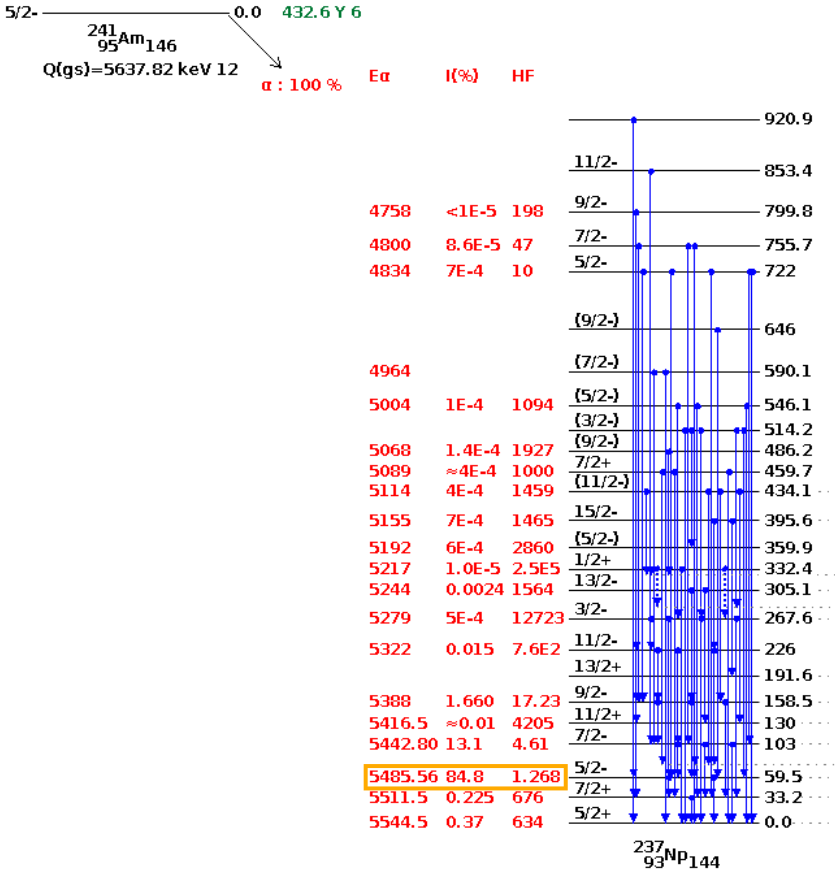
\includegraphics[width=0.7\textwidth]{Thermschema.png}
    \caption{Termschema des $\alpha$-Zerfalls von $^{241}\text{Am}$ zu $^{237}\text{Np}$ (Quelle: National Nuclear Data Center, NuDat 3, \url{https://www.nndc.bnl.gov/nudat3/replotdec.jsp})}
    \label{fig:termschema}
\end{figure}

Wie dem Termschema in Abbildung \ref{fig:termschema} zu entnehmen ist, finden bei diesem Zerfallsprozess verschiedene Übergänge auf unterschiedliche Energieniveaus des Tochterkerns statt. Für die Versuchsdurchführung und Auswertung ist jedoch vor allem der Hauptübergang entscheidend. In $84{,}4\,\%$ der Zerfälle werden $\alpha$-Teilchen mit einer kinetischen Energie von $5485{,}56\,\text{keV}$ emittiert. Da die Intensität der benachbarten Energielinien vergleichsweise gering ist, kann der Strahl in näherungsweise als monoenergetisch betrachtet werden. Diese Startenergie von $E_0 = 5{,}486\,\text{MeV}$ ist der Referenzwert für alle nachfolgenden Berechnungen.

\section{Versuchsaufbau}
\subsection{Streukammer}
Das Americium-241 Präparat befindet sich im Versuch in der zylindrischen Vakuum-Streukammer aus Metall. Einen Überblick über die Laborapparatur liefert Abbildung \ref{fig:aufbau_foto}.

\begin{figure}[htbp]
    \centering
    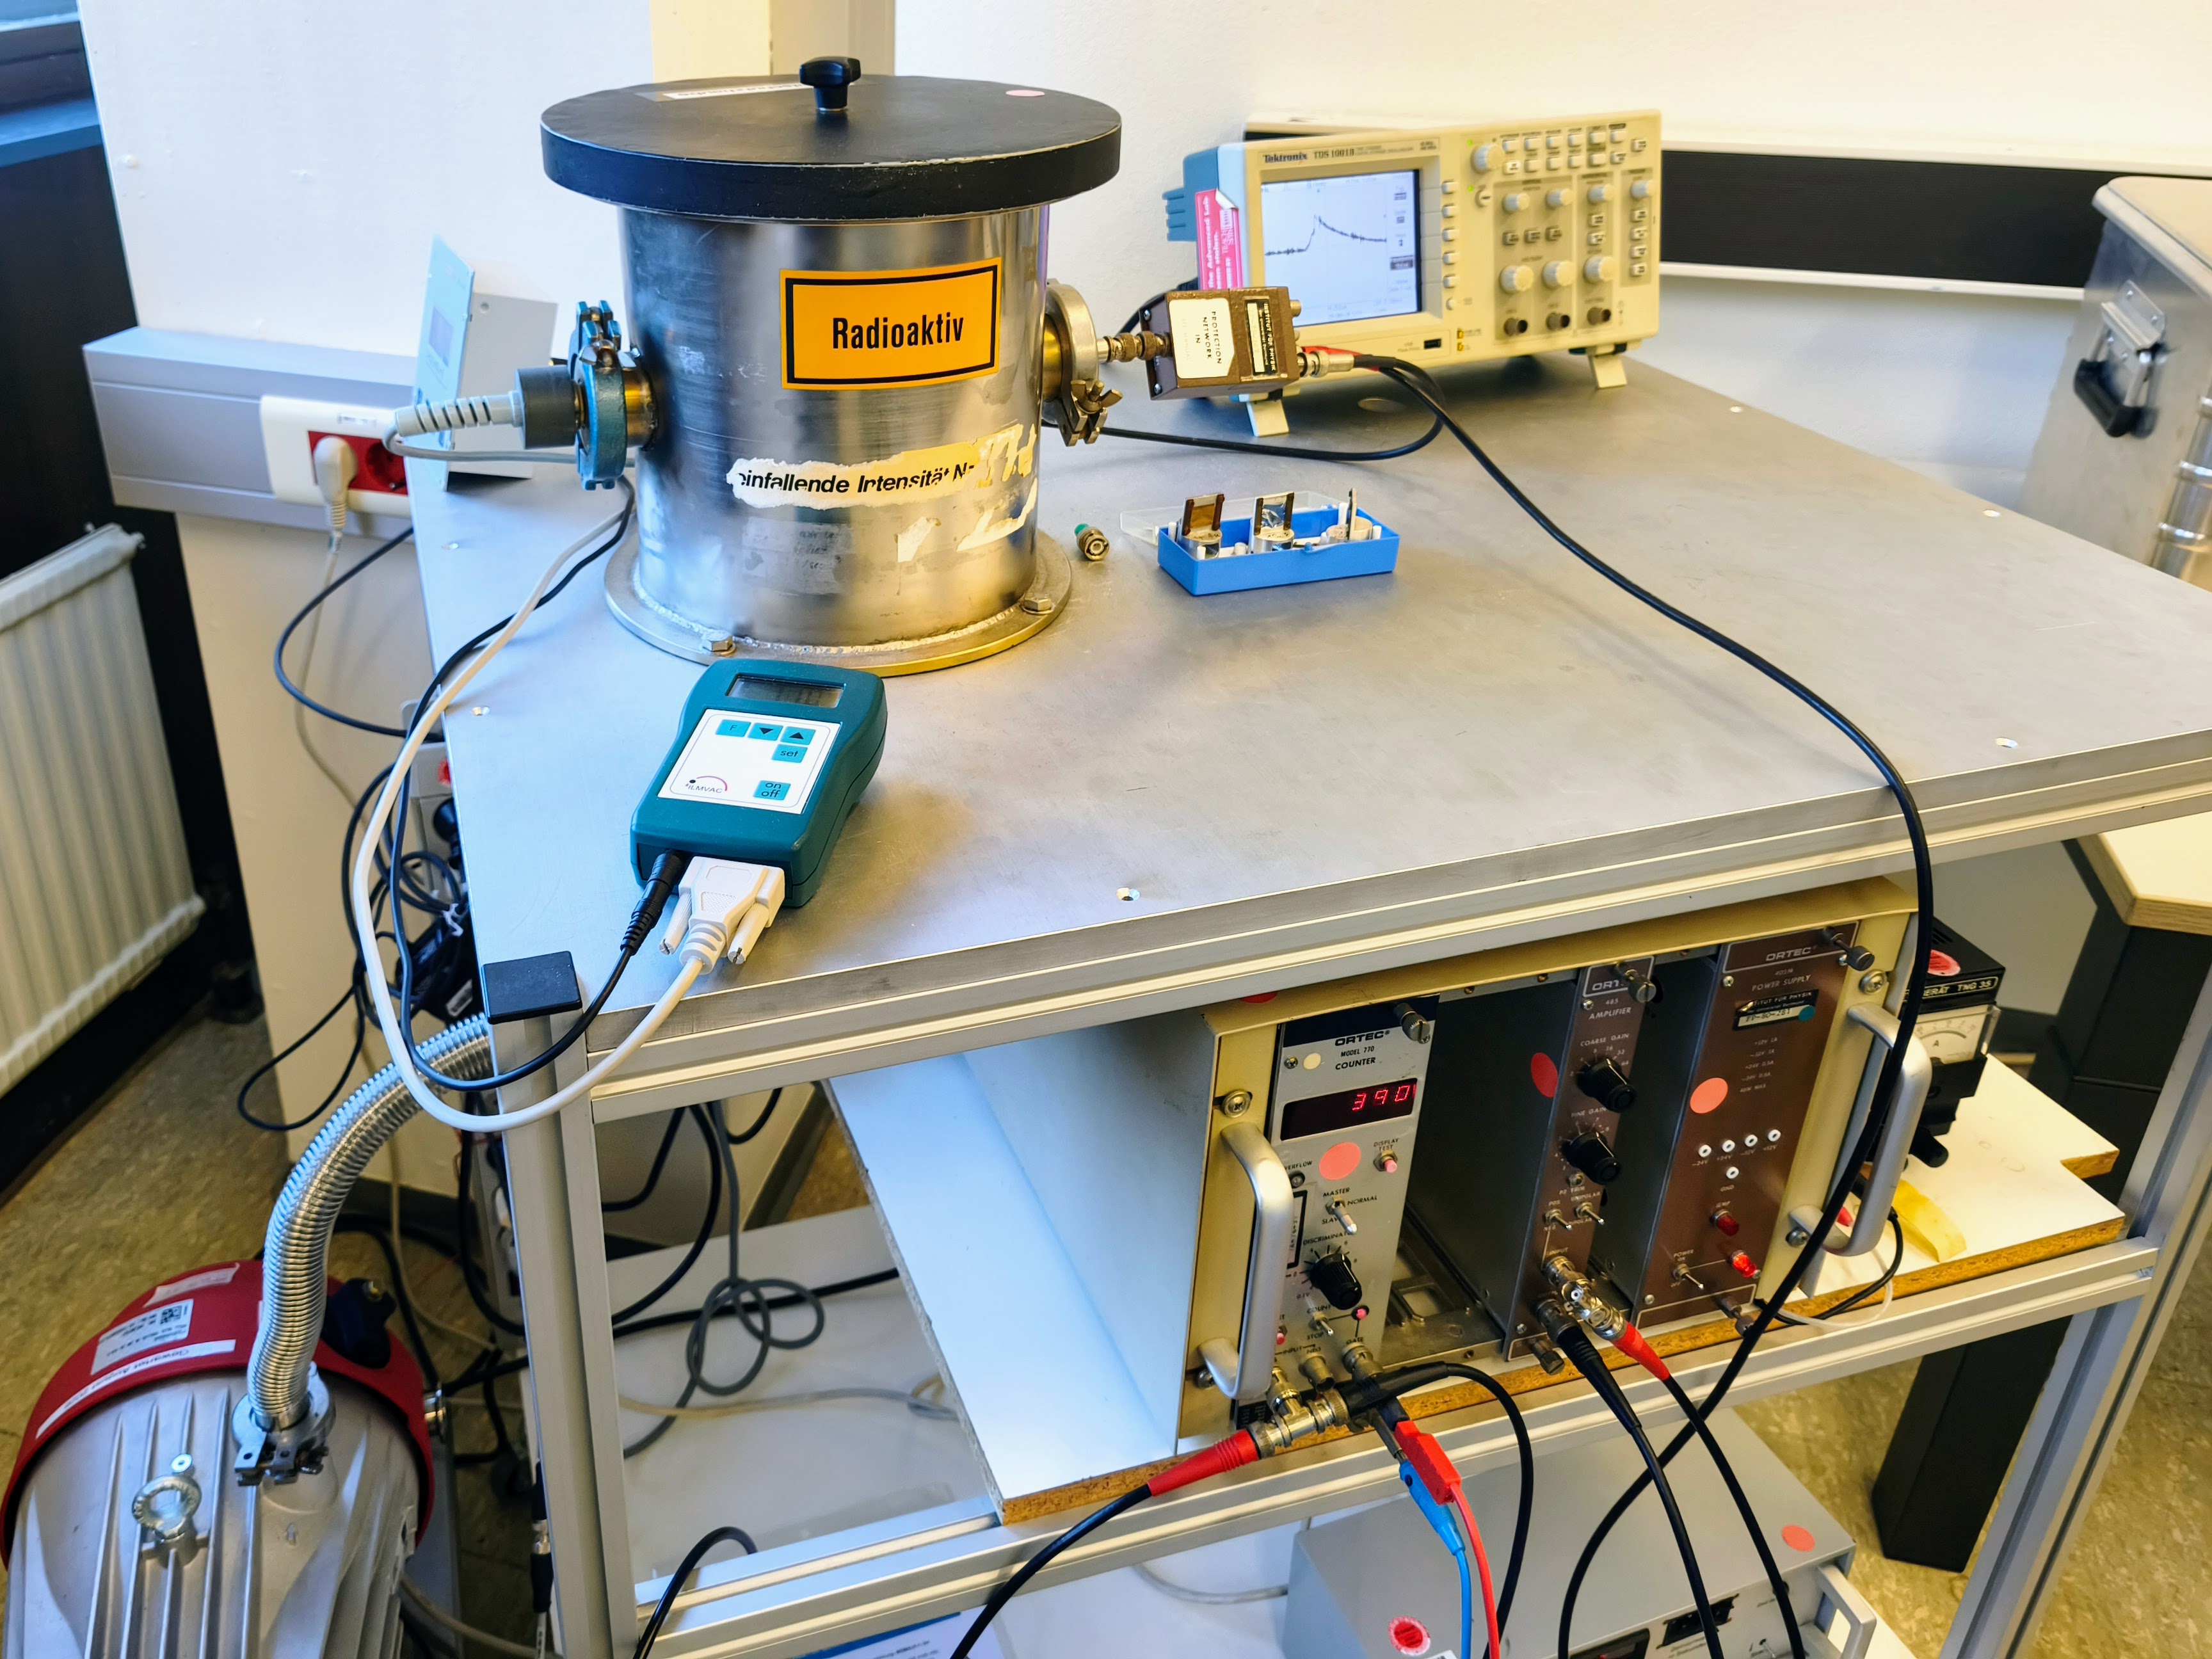
\includegraphics[width=0.8\textwidth]{Aufbau_foto.jpg}
    \caption{\textbf{Aufbau Rutherford Streu-Versuch} }
    In der Mitte befindet sich die zylindrische Vakuumkammer in welcher sich der $\alpha$-Strahler, die Goldfolie und der schwenkbare Detektor befinden. Über einen Metallwellschlauch auf der linken Seite ist die Kammer mit der Scrollpumpe verbunden, der Innendruck wird über ein digitales Handmessgerät überwacht. An der rechten Seite wird das Detektorsignal ausgeleitet und im Oszilloskop visualisiert.
    \label{fig:aufbau_foto}
\end{figure}

Als Quelle dient der $\alpha$-Strahler $^{241}\text{Am}$. Der Strahl trifft im Zentrum der Kammer auf die Goldfolie. Die Detektion der gestreuten Teilchen erfolgt über einen Oberflächensperrschichtzähler, der auf einem Schwenkarm montiert ist. Dieser Arm lässt sich von außen über eine Drehdurchführung rotieren, wobei der eingestellte Streuwinkel $\Theta$ an einer äußeren Skala abgelesen werden kann. 

Die Abmessungen des Strahlengangs sind in der Skizze in Abbildung \ref{fig:abmessungen} zusammengefasst.

\begin{figure}[htbp]
    \centering
    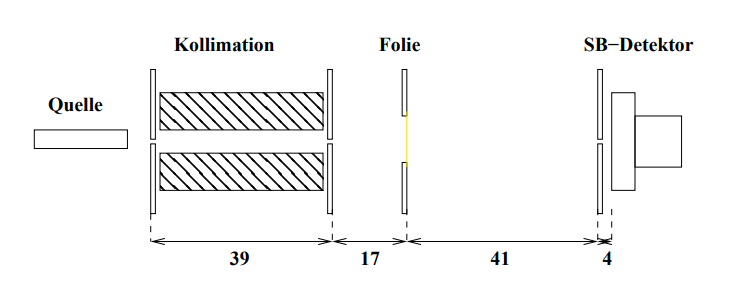
\includegraphics[width=0.8\textwidth]{Abmessungen.png}
    \caption{\textbf{Schematische Darstellung der inneren Streukammer.} 
    Die Abbildung illustriert die geometrischen Abmessungen des Versuchsaufbaus, insbesondere die Distanzen zwischen der Quelle, Goldfolie und dem schwenkbaren Halbleiterdetektor. Entnommen aus \cite{tudoV16}.}
    \label{fig:abmessungen}
\end{figure}

Da die $^{241}\text{Am}$ Quelle in alle Richtungen strahlt, wird der Teilchenstrahl durch zwei rechteckige Schlitzblenden mit der Abmessung $2\,\text{mm} \times 10\,\text{mm}$ kollimiert. Diese Blenden schirmen alle Teilchen ab, die nicht durch die Blende fliegen, und definieren so direkt den effektiven Raumwinkel $\Omega$, den der Detektor abdeckt.
\subsection{Messelektronik und Signalverarbeitung}
Zur Impulserfassung dient ein Silizium-Halbleiterdetektor, spezifisch ein sogenannter Oberflächensperrschichtzähler (Surface Barrier Detector). Die Funktionsweise basiert auf der charakteristischen Bandstruktur von Halbleitern. Ein voll besetztes Valenzband und ein leeres Leitungsband sind durch eine energetisch relativ kleine Bandlücke voneinander getrennt. 
Trifft $\alpha$-Strahlung auf den Detektor, überträgt sie ihre kinetische Energie durch Stoßionisation auf die Elektronen im Valenzband. Diese überwinden die Bandlücke und gelangen in das Leitungsband, wodurch freie Elektronen-Loch-Paare entstehen. Da die Erzeugung eines solchen Paares im Silizium im Mittel eine feste Energie von ca. $3,6\,\text{eV}$ erfordert, ist die Gesamtzahl der generierten primären Ladungsträger direkt proportional zur deponierten Energie der einfallenden Strahlung \footnote{Vgl. Medizinphysik-Wiki: \textit{Halbleiter}, \url{https://medizinphysik.wiki/glossar/halbleiter/}, abgerufen am 08.11.2026.} . 
Damit diese Ladungsträger nicht sofort wieder rekombinieren, wird eine externe elektrische Sperrspannung an den Halbleiter angelegt. Diese verarmt die aktive Zone an freien Ladungsträgern und baut ein elektrisches Feld auf. Die durch das $\alpha$-Teilchen erzeugten Elektronen werden in diesem Feld in entgegengesetzte Richtungen beschleunigt und driften zu den Elektroden, was den messbaren Stromimpuls erzeugt.

Der Impuls wird durch einen Pre-Amplifier integriert und in einen proportionalen Spannungsimpuls umgewandelt. Danach läuft das Signal weiter in den Shape-Amplifier. Dieser verstärkt es nicht nur, sondern formt den anfänglich asymmetrischen Puls in ein sauberes, gaußähnliches Signal um. Diese Pulsformung verbessert das Signal-Rausch-Verhältnis signifikant und verhindert Signalüberlagerungen bei hohen Zählraten. Ganz am Ende wird das fertige Signal aufgeteilt, ein Teil geht in das Oszilloskop. Parallel dazu läuft das Signal in die Zähleinheit. Dort sorgt ein vorgeschalteter Diskriminator dafür, dass das elektronische Hintergrundrauschen einfach abgeschnitten wird, sodass am Ende nur die echten $\alpha$-Teilchen Impulse für die Winkelverteilung gezählt werden.

\subsection{Vakuumsystem und Pumpentechnik}
Um die Streuung der $\alpha$-Teilchen an Luftmolekülen und den damit einhergehenden Energieverlust gemäß der Bethe-Bloch-Gleichung zu minimieren, muss die gesamte Streukammer evakuiert werden. Zur Erzeugung des benötigten Vakuums kommen prinzipiell zwei Arten von Rotationsverdrängerpumpen infrage, die sich in ihrer Funktionsweise und Eignung für sensible Messapparaturen unterscheiden, die Drehschieberpumpe und die Scrollpumpe.

\textbf{Ölgeschmierte Drehschieberpumpe} \\
Die Drehschieberpumpe besteht aus einem zylindrischen Stator, in dessen Innerem sich ein exzentrisch gelagerter Rotor dreht\footnote{Vgl. Jousten, K. (Hrsg.): \textit{Wutz Handbuch Vakuumtechnik}, Springer Vieweg, S. 196.}. Wie in Abbildung \ref{fig:drehschieber} dargestellt, befinden sich in den Schlitzen des Rotors bewegliche Schieber, die durch die Zentrifugalkraft an die Gehäusewand gedrückt werden. Diese Schieber unterteilen den Raum in sich verändernde, sichelförmige Schöpfräume. Das einströmende Gas wird eingeschlossen, durch die Rotation des Rotors verdichtet und schließlich durch ein Auslassventil ausgestoßen\footnote{Vgl. Wutz, ebd.}. Um die feinen Spalte zwischen Rotor, Schieber und Stator effektiv abzudichten, wird in diesen Pumpen ein hochwertiges Mineralöl als Betriebsmittel eingesetzt. Durch diese Öldichtung erreichen einstufige Ausführungen zuverlässig Enddrücke im Feinvakuumbereich von typischerweise $0,1\,\text{hPa}$ bis $20\,\text{hPa}$\footnote{Vgl. Wutz, S. 198.}.

\begin{figure}[htbp]
    \centering
    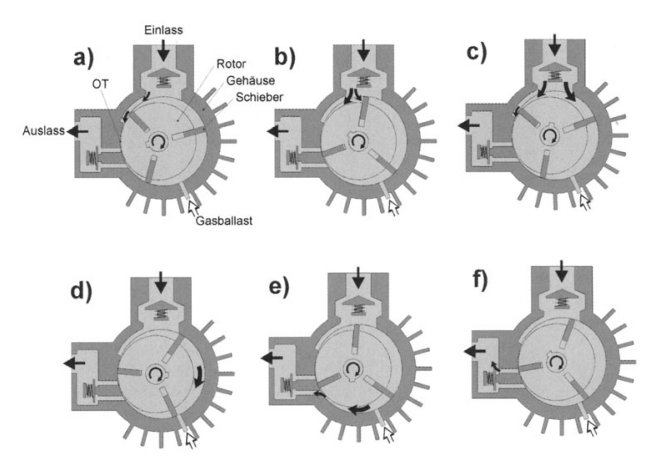
\includegraphics[width=0.8\textwidth]{Drehschieberpumpe.png}
    \caption{\textbf{Funktionsprinzip einer einstufigen Drehschieberpumpe in sechs Phasen (a–f).} 
    Die schematische Darstellung zeigt den Arbeitszyklus, bestehend aus Ansaugen, Verdichten und Ausstoßen des Gases. (a–c) Ansaugphase: Das Volumen der saugseitigen Zelle vergrößert sich, wodurch Gas durch den Einlass in die Pumpe strömt. (d) Verdichtungsphase: Die Schöpfzelle ist vom Einlass getrennt; das eingeschlossene Gasvolumen wird durch die weitere Rotation komprimiert. (e) Gasballast-Zufuhr. (f) Ausstoßphase: Das komprimierte Gas-Dampf-Gemisch öffnet das Auslassventil gegen den atmosphärischen Druck und wird ausgestoßen.}
    \label{fig:drehschieber}
\end{figure}

Trotz der hohen Zuverlässigkeit und Langlebigkeit besitzt die Ölschmierung für das Rutherford-Experiment den entscheidenden Nachteil, dass Hoch- und Feinvakuumbereich  Öldämpfe entgegen der Pumprichtung in die Messkammer zurückströmen können. Dieser Dampf kann sich im Raum ausbreiten und im schlechtesten Fall die Messung beeinträchtigen. 

\textbf{Scrollpumpe} \\
Eine Alternative bietet die Scrollpumpe, deren Verdichtungsprinzip auf zwei ineinandergreifenden archimedischen Spiralen beruht\footnote{Vgl. Wutz, S. 210.}. Während eine der Spiralen starr im Gehäuse fixiert ist, führt die zweite Spirale eine zentralsymmetrische, oszillierende Bewegung das sogenannte Orbitieren aus\footnote{Vgl. Wutz, ebd.}. Durch diese exzentrische Relativbewegung entstehen halbmondförmige Gasvolumina, die das Gas kontinuierlich von der Außenseite in das Zentrum der Spirale fördern und dort in Richtung des Auslasses verdichten\footnote{Vgl. Wutz, S. 210-211.} (siehe Abbildung \ref{fig:scroll}).

\begin{figure}[htbp]
    \centering
    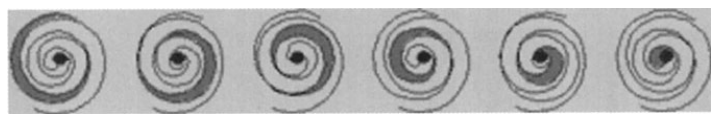
\includegraphics[width=0.8\textwidth]{Scrollpumpe.png}
    \caption{\textbf{Der Weg des Gases in der Scroll-Spirale.} 
    Die Abbildung zeigt das Verdichtungsprinzip durch zwei ineinandergreifende archimedische Spiralen. Durch die zentralsymmetrische Oszillation (Orbitieren) der beweglichen Spirale gegenüber der feststehenden Spirale wird das einströmende Gas am äußeren Rand in halbmondförmigen Volumina eingeschlossen. Diese Gastaschen wandern kontinuierlich in das Zentrum der Spirale, wodurch der Druck stetig ansteigt, bis das verdichtete Gas schließlich durch die zentrale Auslassöffnung ausgestoßen wird.}
    \label{fig:scroll}
\end{figure}

Der Vorteil dieses Pumpentyps ist der absolut trockenlaufende und ölfreie Betrieb. Die dynamische Abdichtung der Kammern erfolgt hierbei nicht durch Flüssigkeiten, sondern rein durch minimale Fertigungstoleranzen der Spiralwände sowie durch flexible Kunststoffdichtungen an den Stirnflächen\footnote{Vgl. Wutz, S. 211.}. Scrollpumpen erreichen Enddrücke im Bereich von ca. $10^{-2}\,\text{hPa}$ und reichen damit nicht ganz an die extremen Vakuumwerte mehrstufiger ölgeschmierter Pumpen heran\footnote{Vgl. Wutz, S. 212.}. Dafür gewährleisten sie jedoch eine vollständig kohlenwasserstofffreie Evakuierung. Für die Evakuierung der Streukammer kam im Versuch eine trockene Scroll-Vakuumpumpe vom Typ Pfeiffer Vacuum HiScroll 18 (DN 25 ISO-K) zum Einsatz, welche am Pumpenstand laut Anzeige einen minimalen Druck von $1,4 \cdot 10^{-1}\,\text{mbar}$ ($0,14\,\text{hPa}$) erreichte. Die eigentlichen Messreihen wurden im Versuch jedoch bereits ab einem stabilisierten Kammerdruck von ca. $10\,\text{mbar}$ ($10\,\text{hPa}$) begonnen. Die Restgasdichte ist bei diesem Druck bereits so reduziert, dass der Energieverlust der $\alpha$-Teilchen auf der kurzen Flugstrecke zwischen Streuzentrum und Detektor gemäß der Bethe-Bloch-Gleichung vernachlässigt werden kann.
\section{Durchführung}
Am Anfang der Messungen wurde die Sperrspannung des Halbleiterdetektors auf $12\,\text{V}$ eingestellt und die Strahlungsquelle hochgefahren. Zudem wurde am Oszilloskop als Grundeinstellung die Mittelwert-Funktion eingestellt, um das Signal zu glätten.
Damit das elektronische Hintergrundrauschen von den Messsignalen getrennt ist, wurde als Erstes der Diskriminator justiert. Dazu wurde die Diskriminatorschwelle schrittweise erhöht, bis auf dem Oszilloskop keine kleinen Amplituden mehr zu sehen waren. Dieser Zustand wurde bei einem Schwellenwert von 6 erreicht.
Im Anschluss wurden die charakteristischen Signalbilder am Oszilloskop aufgenommen. Dabei wurde das ursprüngliche Signal direkt aus dem Pre-Amplifier mit dem Puls nach dem Shape-Amplifier optisch verglichen und dokumentiert.

Vor der eigentlichen Streumessung an der Goldfolie wurde zunächst der ungestörte Primärstrahl vermessen. Ziel war es, das Strahlprofil aufzunehmen und die maximale einfallende Intensität $I_0$ zu bestimmen. Diese ungestörte Intensität wird benötigt, um die experimentelle Aktivität der $^{241}\text{Am}$-Quelle berechnen zu können.
Dazu wurde der Detektor ohne eingesetzte Folie in kleinen Winkelschritten in die positive und negative Richtung um den vorläufigen mechanischen Nullpunkt herum geschwenkt. Um die statistische Unsicherheit gering zu halten, wurde für die Messintervalle nach Möglichkeit eine Ereigniszahl von mindestens $1111$ Counts angepeilt. Nach der Poisson-Statistik ($\Delta N / N = 1/\sqrt{N}$) entspräche dies einem angestrebten relativen Fehler von $3\,\%$. 
Aus den notierten Messzeiten und Counts ergab sich eine gaußförmige Zählratenverteilung. Das Maximum dieser Gaußkurve markiert das Zentrum und die höchste Intensität des Primärstrahls. An der gefundenen Maximumsposition wurde die Winkelskala der Apparatur direkt physisch auf $0^\circ$ neu kalibriert. Dadurch entsprach bei den darauffolgenden Messungen der abgelesene Winkel dem wahren Streuwinkel.

Nach der Kalibrierung wurde die Goldfolie in den Strahlengang eingesetzt. Für die Rutherford-Messung wurde der Detektor auf Winkel außerhalb des soeben ausgemessenen Primärstrahl-Intervalls eingestellt. Hier wurden für verschiedene Winkel in positive Richtung Counts $N$ und Messdauer erfasst.

Um die Bethe-Bloch-Gleichung experimentell zu überprüfen und die genaue Dicke der Goldfolie zu ermitteln, wurde abschließend die Druckabhängigkeit des Energieverlusts der $\alpha$-Teilchen gemessen. Ausgehend von einem Kammerdruck von etwa $10\,\text{mbar}$ wurde der Druck stetig erhöht. Bei jedem Druckschritt wurde die maximale Spannungsamplitude am Oszilloskop abgelesen, woraus sich die Restenergie der Teilchen ergibt. Diese Messreihe wurde so lange fortgeführt, bis die Spannung konstant blieb und die Teilchen im Gasgemisch vollständig abgebremst wurden. Dieser Vorgang wurde zweimal durchgeführt, einmal mit und einmal ohne Goldfolie.
\section{Auswertung}

\subsection {Darstellung am Oszilloskop}

Die durch den Surface-Barrier-Detektor detektierten Signale werden grundsätzlich durch einen Preamplifier verstärkt.\\
In \autoref{fig:oszill_unver} ist der so aufgenommene Spannungsimpuls, verursacht durch auf den Detektor auftreffende $\alpha$-Teilchen, dargestellt.\\
Es sind deutliche Artefakte zu sehen, was das Auslesen der Spannung fehleranfällig machen kann.

\begin{figure}[H]
    \centering
    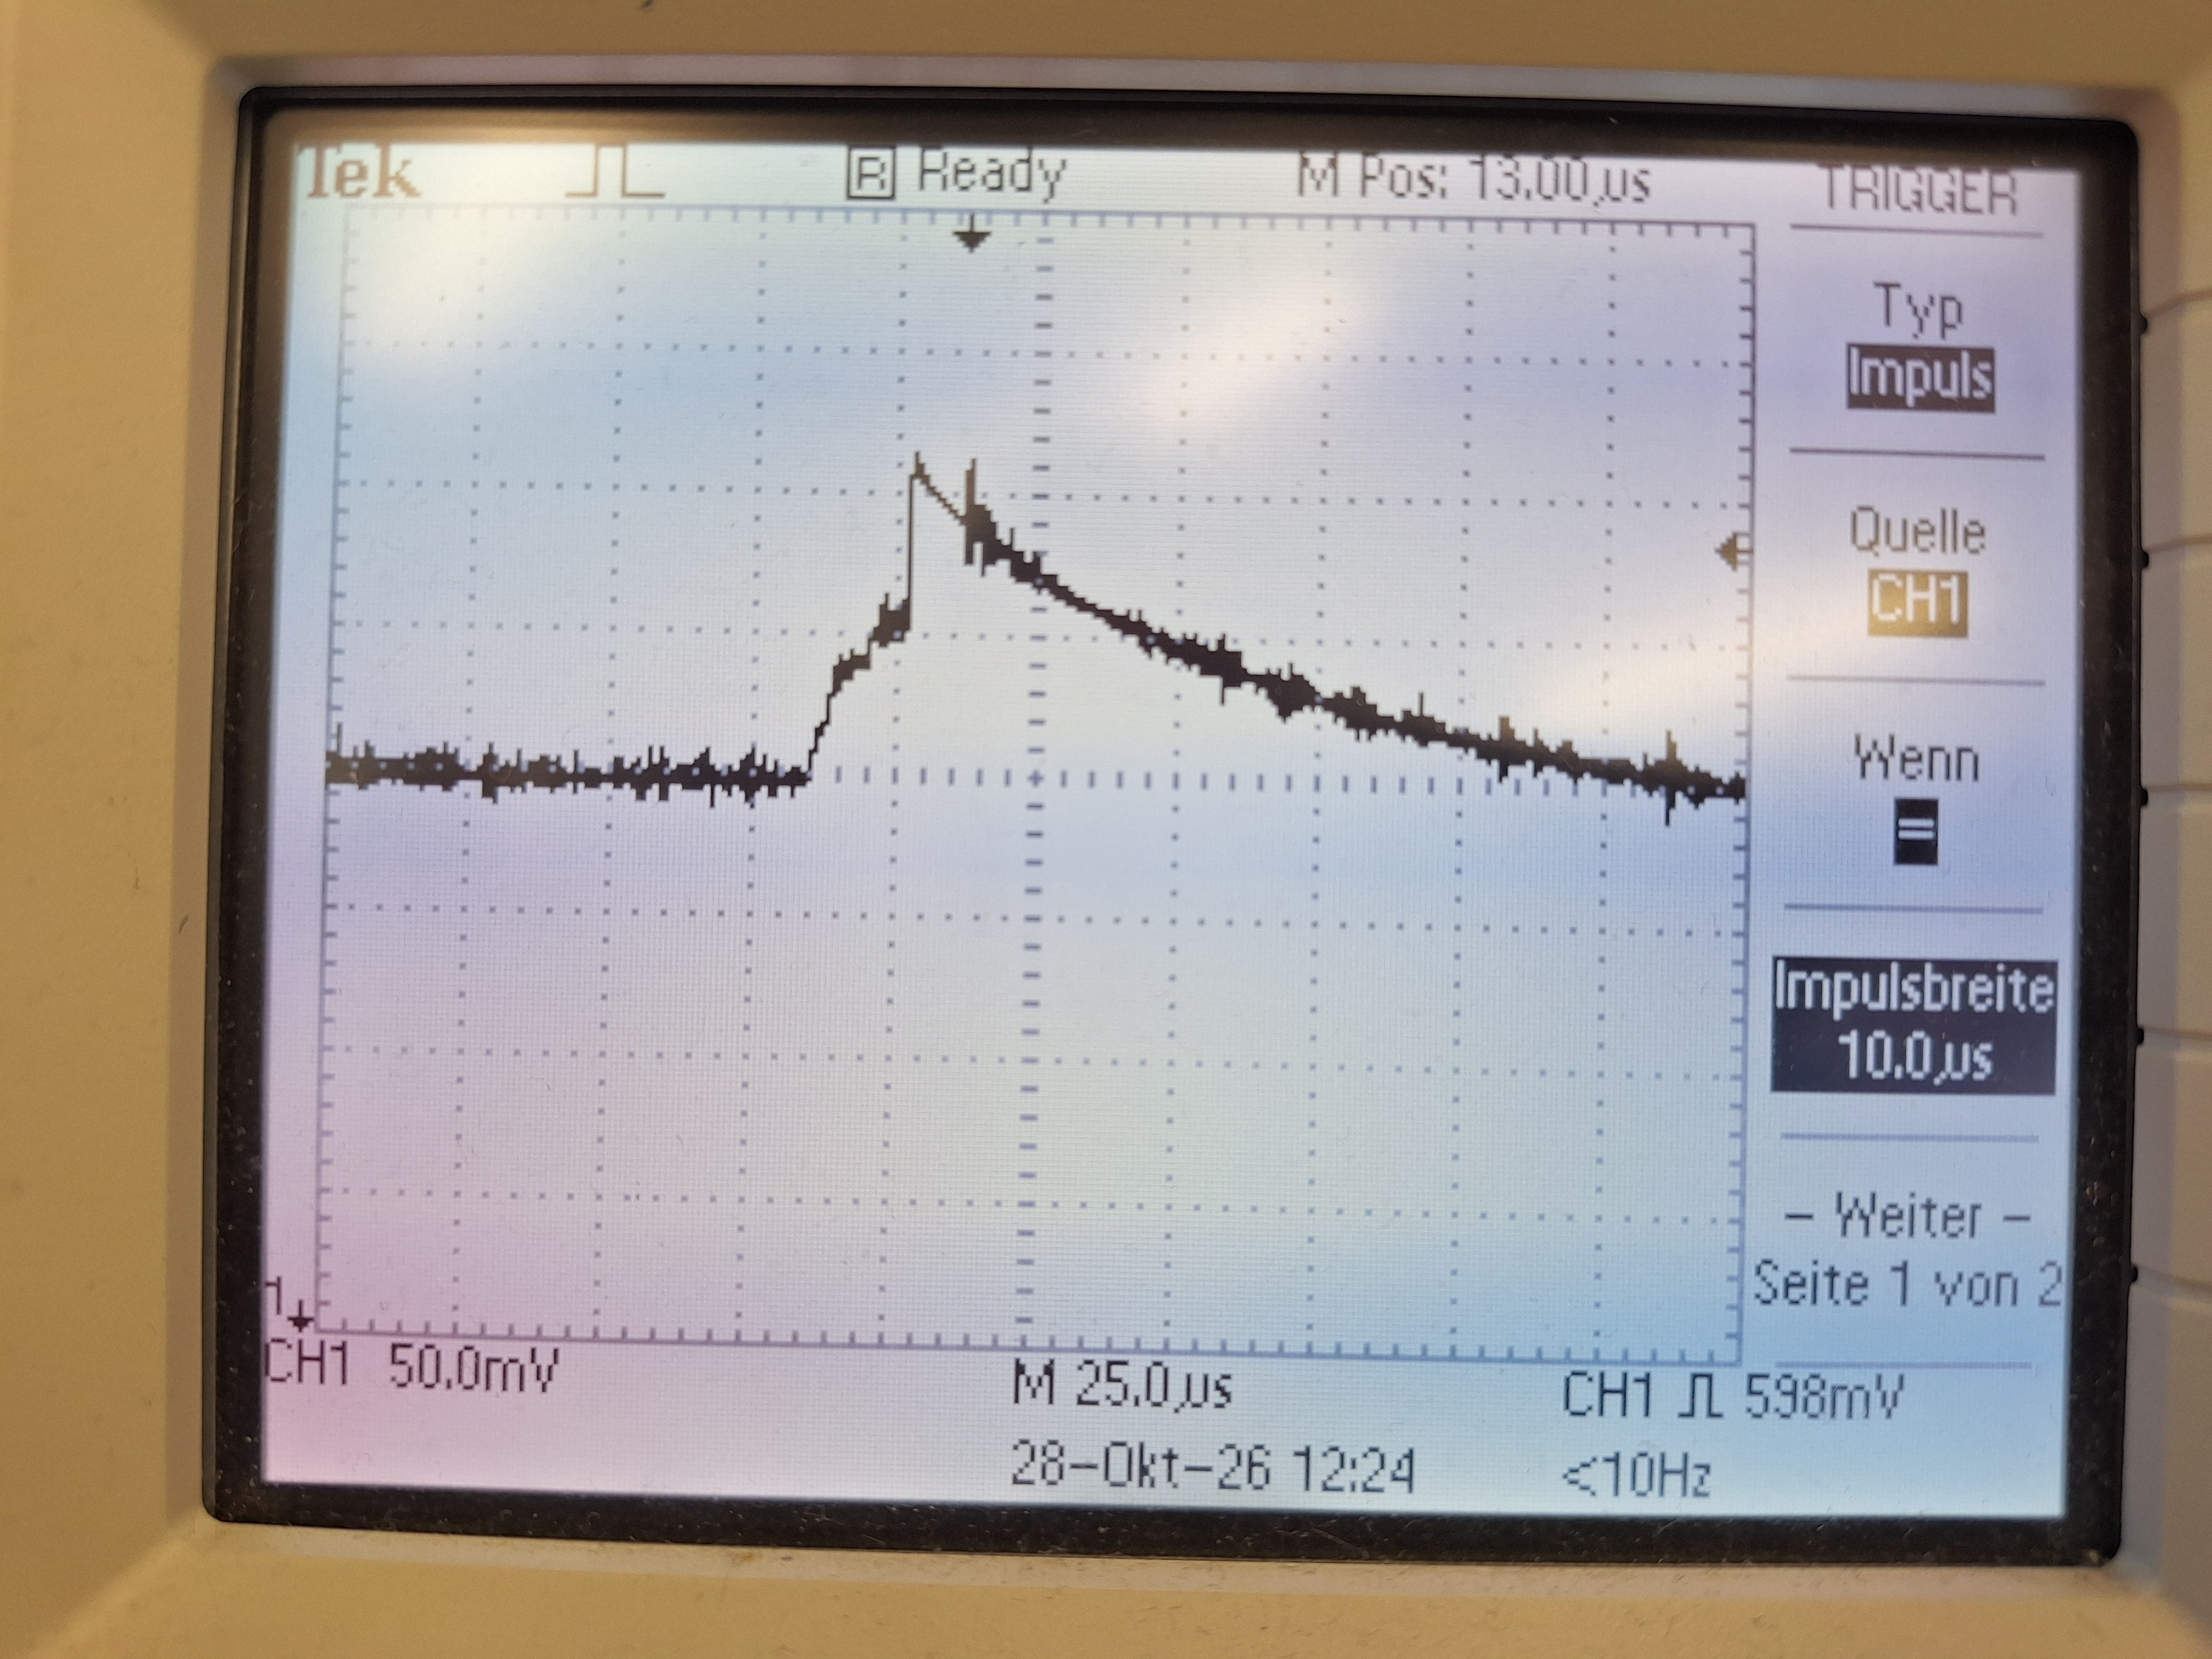
\includegraphics[width=0.7\textwidth]{images/unverstaerkt.jpg}
    \caption{Ausgabe des Oszilloskops mit Preamplifier}
    \label{fig:oszill_unver}
\end{figure}

Unter Zuschaltung eines Shape-Amplifiers lässt sich das ebengenannte Problem beheben, die vom Oszilloskop aufgenommene Kurve, dargestellt in \autoref{fig:oszill_ver}, 
erscheint geglättet und ist geeignet, nachfolgende Messungen im Rahmen dieses Versuchs durchzuführen.

\begin{figure}[H]
    \centering
    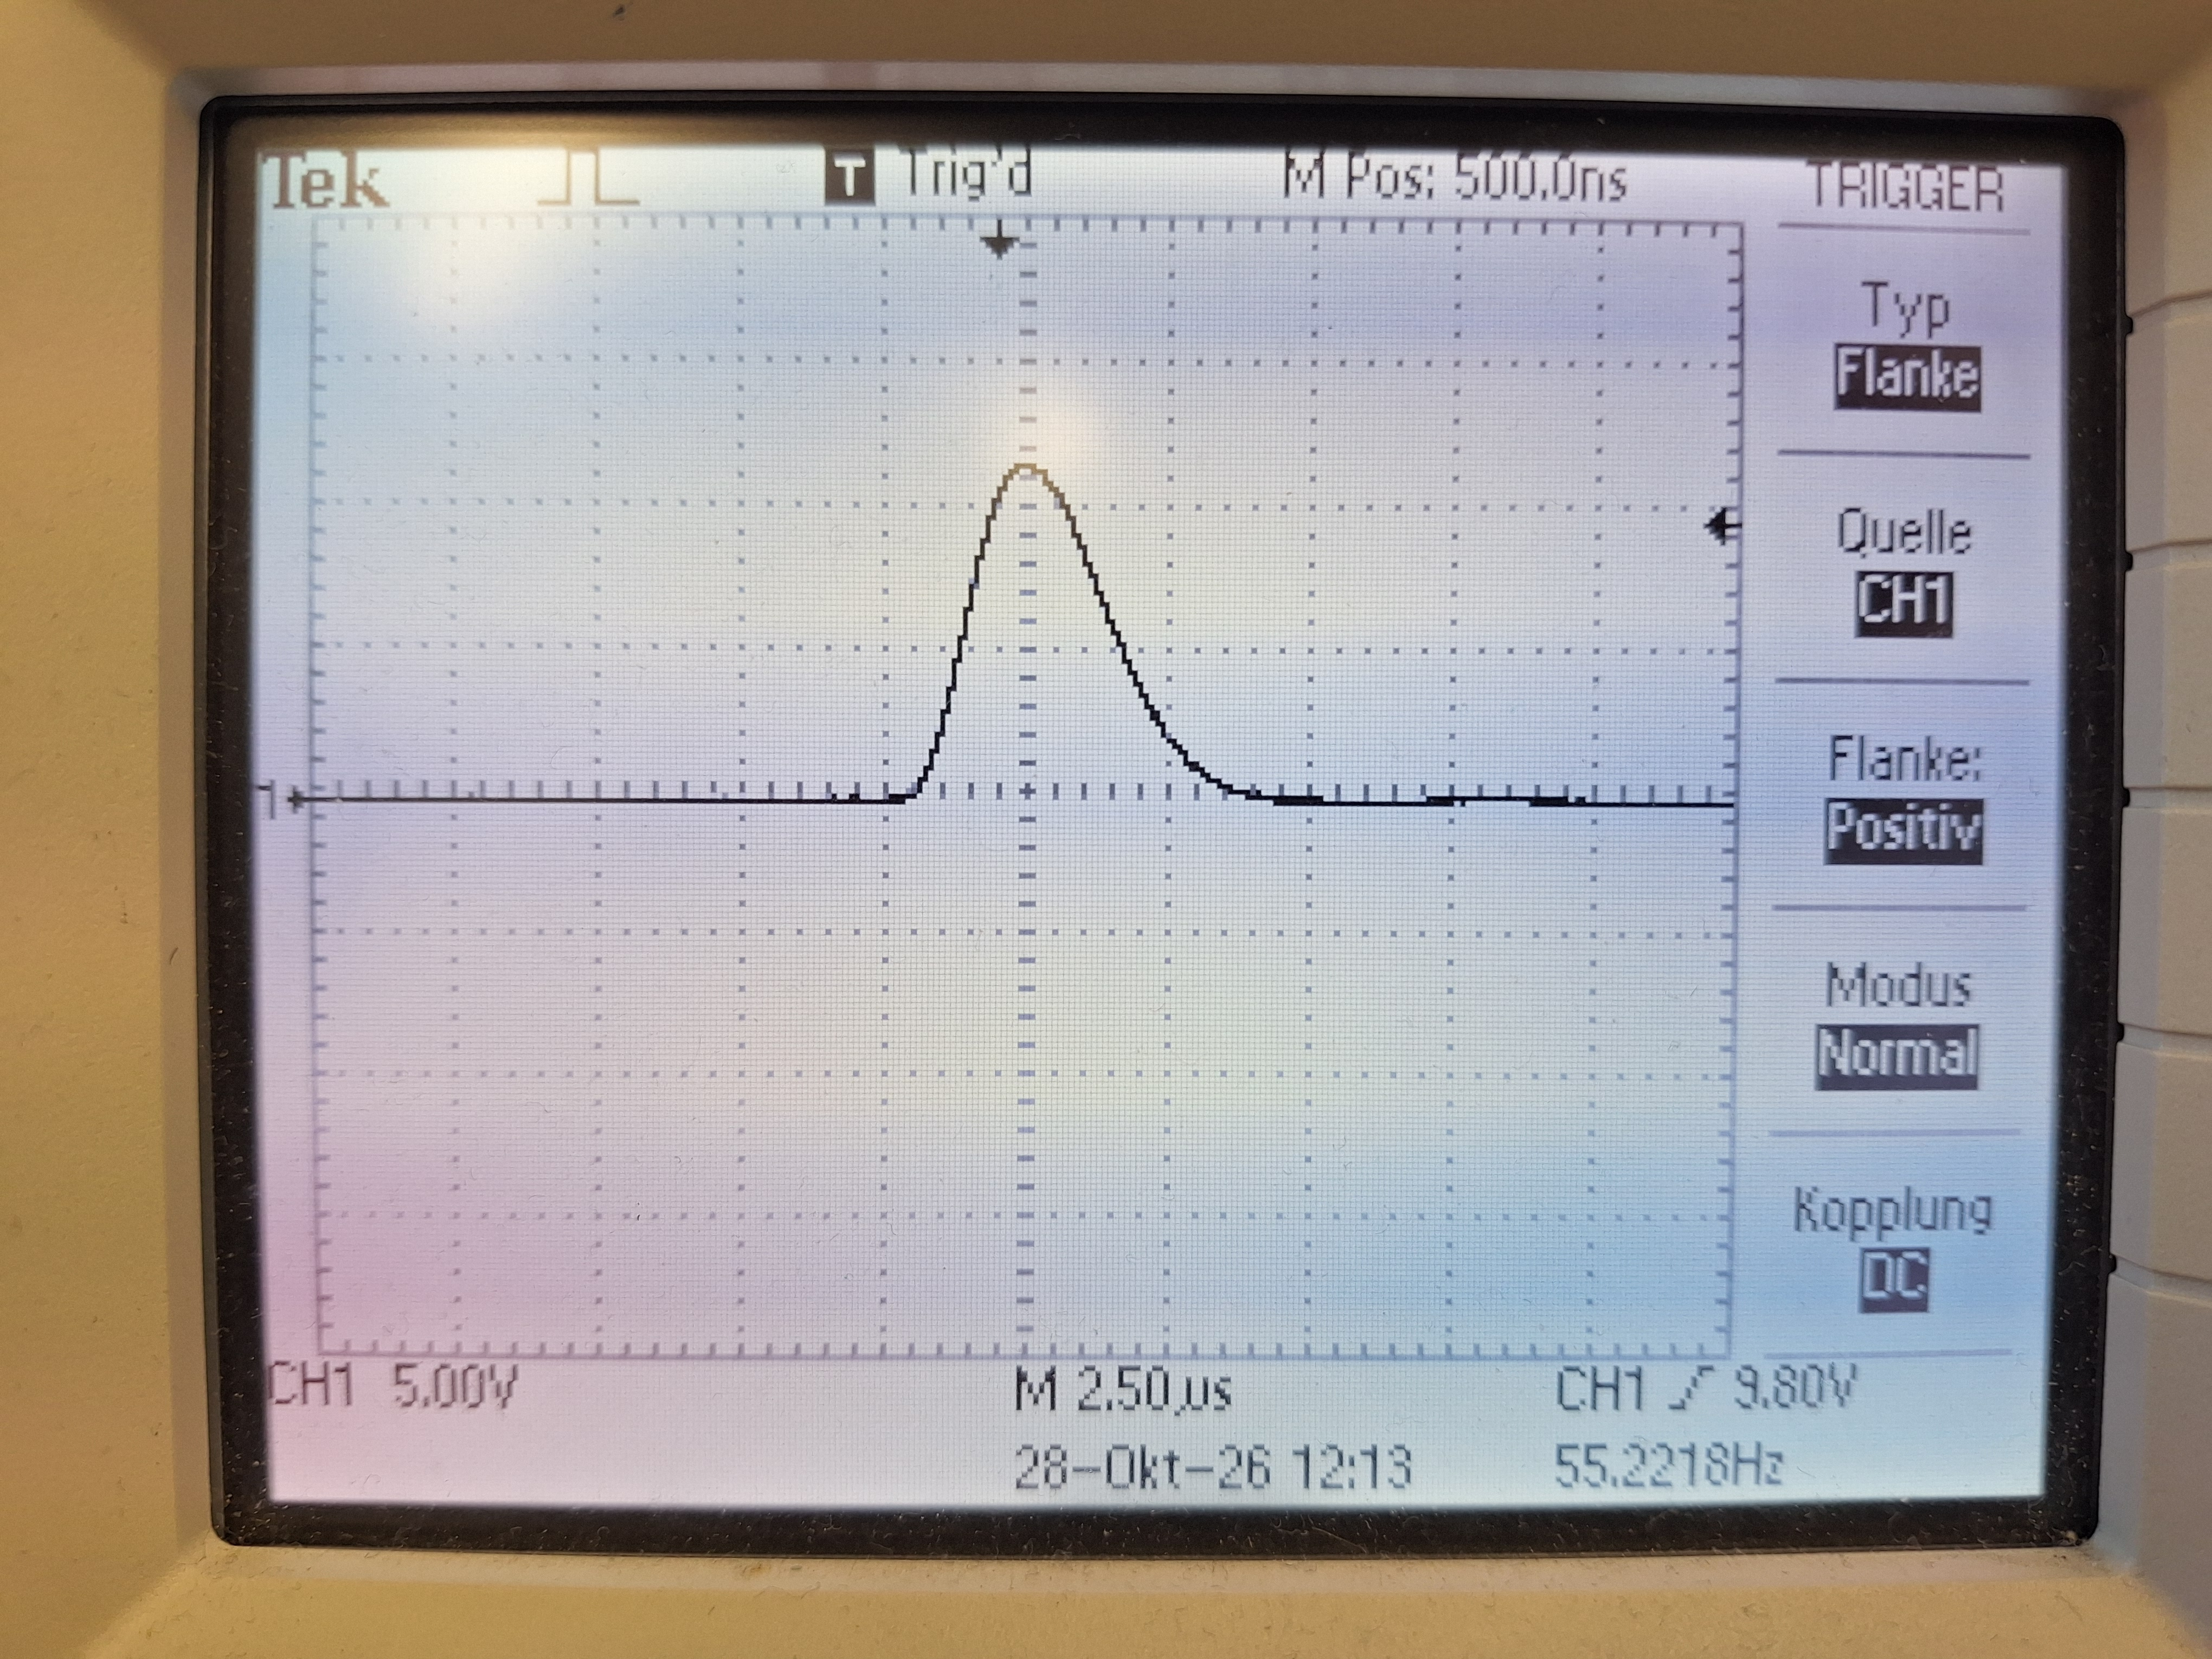
\includegraphics[width=0.7\textwidth]{images/verstaerkt.jpg}
    \caption{Ausgabe des Oszilloskops mit Preamplifier und nachgeschaltetem Shaping Amplifier}
    \label{fig:oszill_ver}
\end{figure}

Für die folgenden Messungen wurde auf positive Flanke getriggert und der Mittelwert-Funktion für 16 Impulse gewählt.









\subsection{Strahlungsprofil und Winkelkalibrierung}
\label{subsec:kalibrier}

Im vorliegenden Versuchsteil wird vorbereitend ein Strahlungsprofil des kollimierten $\alpha$-Teilchenstrahls in Abhängigkeit verschiedener eingestellter Winkel aufgenommen,
um die maximale Zählrate und damit die Winkeleinstellung zu finden, unter der die Teilchen annähernd senkrecht auf den Detektor treffen.\\
Es wird eine gaußförmige Verteilung der Zählraten erwartet. Die in \autoref{tab:strahlungsprofil} aufgelisteten Messwerte mitsamt ihres für die Zählrate gültigen Poissonfehlers
$\Delta R = \frac{\sqrt{N}}{t}$ sind in \autoref{fig:strahlprofil_plot} dargestellt, wobei entsprechend mit einer gaußförmigen Ausgleichskurve gefittet wird.\\




\begin{table}[htbp]
    \centering
    \resizebox{0.7\textwidth}{!}{%
    \begin{tabular}{cccc}
    \toprule
    Winkel $\theta$ / $\si{\degree}$ & Teilchenzahl $N$ & Messzeit $t$ / $\si{\second}$ & Zählrate $R$ / $\mathrm{s}^{-1}$ \\
    \midrule
    -3.0 & $1157 \pm 34.0$ & 1000 & $1.157 \pm 0.034$ \\
    -2.0 & $1119 \pm 33.5$ & 210 & $5.329 \pm 0.159$ \\
    -1.5 & $1192 \pm 34.5$ & 140 & $8.514 \pm 0.247$ \\
    -1.0 & $1114 \pm 33.4$ & 103 & $10.816 \pm 0.324$ \\
    -0.5 & $1110 \pm 33.3$ & 81 & $13.704 \pm 0.411$ \\
    0.0 & $1113 \pm 33.4$ & 69 & $16.130 \pm 0.484$ \\
    0.5 & $1145 \pm 33.8$ & 63 & $18.175 \pm 0.537$ \\
    1.0 & $1113 \pm 33.4$ & 62 & $17.952 \pm 0.538$ \\
    1.5 & $1120 \pm 33.5$ & 60 & $18.667 \pm 0.558$ \\
    2.0 & $1123 \pm 33.5$ & 60 & $18.717 \pm 0.559$ \\
    2.5 & $1135 \pm 33.7$ & 66 & $17.197 \pm 0.510$ \\
    3.0 & $1186 \pm 34.4$ & 65 & $18.246 \pm 0.530$ \\
    3.5 & $1132 \pm 33.6$ & 69 & $16.406 \pm 0.488$ \\
    4.0 & $1152 \pm 33.9$ & 75 & $15.360 \pm 0.453$ \\
    4.5 & $1117 \pm 33.4$ & 90 & $12.411 \pm 0.371$ \\
    5.0 & $1125 \pm 33.5$ & 120 & $9.375 \pm 0.280$ \\
    6.0 & $1118 \pm 33.4$ & 275 & $4.065 \pm 0.122$ \\
    7.0 & $1163 \pm 34.1$ & 2080 & $0.559 \pm 0.016$ \\
    \bottomrule
    \end{tabular}
    }
    \caption{Messwerte des aufgenommenen Strahlungsprofils.}
    \label{tab:strahlungsprofil}
\end{table}

\begin{figure}[H]
    \centering
    \includegraphics[width=0.9\textwidth]{strahlungsprofil.png}
    \caption{Zählraten in Abhängigkeit vom Messwinkel}
    \label{fig:strahlprofil_plot}
\end{figure}


Das Maximum der Ausgleichskurve liegt bei

\[
\theta_{\max} = (1{,}909 \pm 0{,}006)^\circ
\]

und wurde wie die Kurve mit \textit{SciPy} berechnet.\\
Es wurde für nachfolgende Messungen ein Winkel von $\theta = 1{,}9^\circ$ als kalibrierter Nullwinkel gewählt.

\subsection{Aktivität der Americium-241-Probe}
\label{subsec:aktivitaet}

Nun wird die Aktivität der vorliegenden Americium-241-Probe experimentell bestimmt und mit dem erwarteten Wert verglichen.\\
Die theoretische Aktivität der Probe berechnet sich anhand des radioaktiven Zerfallsgesetzes \eqref{eq:zerfallsgesetz}.
Hier sind die Zerfallskonstante $\lambda = 5{,}077 \cdot 10^{-11}\,\mathrm{s}^{-1}$ \cite{zerfallskonstante}, eine Anfangsaktivität $A_0$ und die seitdem verstrichene Zeit $t$  gemäß der Versuchsanleitung \cite{tudoV16} verwendet, sodass die Aktivität am Tag des durchgeführten Versuchs zu

\[
A_{\mathrm{theo}} = 313{,}5\,\si{\kilo\becquerel}
\]

berechnet wird.\\
Die experimentelle Bestimmung der Probenaktivität erfolgt über Extrapolation der in \autoref{subsec:kalibrier} erfassten Zählrate im dort bestimmten Nullwinkel
auf den gesamten Raumwinkel.
Es wird die dort bestimmte Zählrate $R = (18{,}717 \pm 0{,}559)\,\mathrm{s}^{-1}$beim Winkel $\theta = 2{,}0^\circ$ als größte gemessene Zählrate verwendet.\\
Zur Berechnung wird die Formel 

\[
A_{\mathrm{exp}} = \frac{4\pi R}{\Delta\Omega}
\]

verwendet, wobei für 

\[
\Delta\Omega = \frac{x\,y}{d^2}
\]

angesetzt wird. Die Werte $x = 2 \cdot 10^{-3}\,\mathrm{m}$ und $y = 10 \cdot 10^{-3}\,\mathrm{m}$ entsprechen den Abmessungen der Blende des Kollimators und $d = 1{,}01 \cdot 10^{-1}\,\mathrm{m}$ der Distanz zwischen Strahlungsquelle und Detektor \cite{tudoV16}\\.
Die so bestimmte Aktivität der Americium-241-Probe lautet

\[
A_{\mathrm{exp}} = (120{,}0 \pm 3{,}6)\,\mathrm{kBq}.
\]











\subsection{Bestimmung der Foliendicke}
\label{subsec:dicke}

Im nächsten Versuchsteil wird die Dicke der im nachfolgenden Rutherford'schen Streuexperiment verwendeten Goldfolie experimentell bestimmt.\\
Die mit dem Oszilloskop bei steigenden Kammerdrücken ausgelesenen Spannungsimpulse sind für den Versuch ohne Folie in \autoref{tab:spannung_ohne_folie} und für den Versuch mit Folie in \autoref{tab:spannung_mit_folie} angegeben.\\
Eine graphische Darstellung der aufgenommenen Messwerte inklusive Ausgleichsgeraden ist in \autoref{fig:energieverlust} zu sehen.\\



\begin{table}[htbp]
    \centering
    \resizebox{0.7\textwidth}{!}{%
    \begin{tabular}{cc}
    \toprule
    Kammerdruck $p$ / mbar & Spannungsimpuls $U$ / V \\
    \midrule
    10.7 & 11.4 \\
    21.3 & 11.0 \\
    33.1 & 10.6 \\
    43.6 & 10.6 \\
    71.2 & 9.6 \\
    104.5 & 8.8 \\
    137.2 & 7.6 \\
    179.3 & 6.8 \\
    206.1 & 6.6 \\
    263.2 & 6.4 \\
    320.2 & 6.4 \\
    \bottomrule
    \end{tabular}
    }
    \caption{Spannungsimpulse in Abhängigkeit vom Kammerdruck ohne Folie.}
    \label{tab:spannung_ohne_folie}
\end{table}


\begin{table}[htbp]
    \centering
    \resizebox{0.7\textwidth}{!}{%
    \begin{tabular}{cc}
    \toprule
    Kammerdruck $p$ / mbar & Spannungsimpuls $U$ / V \\
    \midrule
    10.2 & 7.2 \\
    14.9 & 7.0 \\
    34.9 & 7.0 \\
    47.7 & 6.8 \\
    66.4 & 6.8 \\
    90.1 & 6.6 \\
    125.9 & 6.6 \\
    307.8 & 6.4 \\
    716.4 & 6.4 \\
    \bottomrule
    \end{tabular}
    }
    \caption{Spannungsimpulse in Abhängigkeit vom Kammerdruck mit Folie.}
    \label{tab:spannung_mit_folie}
\end{table}

\begin{figure}[H]
    \centering
    \includegraphics[width=0.9\textwidth]{druck_spannung_mit_ohne_folie.png}
    \caption{Spannungsimpulse in Abhängigkeit vom Kammerdruck}
    \label{fig:energieverlust}
\end{figure}


Die Parameter der Ausgleichsgeraden in der Form 

\[
U(p) = a \cdot p + b
\]

lauten 

\[
\begin{array}{rcl@{\qquad}rcl}
a_{\mathrm{ohne}} &=& (-0{,}018 \pm 0{,}002)\,\frac{\mathrm{V}}{\mathrm{mbar}}
&
b_{\mathrm{ohne}} &=& (11{,}0 \pm 0{,}3)\,\mathrm{V}
\\[6pt]
a_{\mathrm{mit}} &=& (-0{,}0009 \pm 0{,}0003)\,\frac{\mathrm{V}}{\mathrm{mbar}}
&
b_{\mathrm{mit}} &=& (6{,}9 \pm 0{,}1)\,\mathrm{V}
\end{array}
\]

Mit diesen kann nun der für die nachfolgende Berechnung verwendete Energieverlust der Alphateilchen $\Delta E$ beim Durchgang durch die Folie gemäß

\[
\Delta E = E_{\alpha}\left(1-\frac{b_{\mathrm{mit}}}{b_{\mathrm{ohne}}}\right)
\]

berechnet werden, wobei $E_{\alpha} = 5{,}486\,\mathrm{MeV}$ gemäß \eqref{eq:zerfallsgesetz} verwendet wird.
Es ergibt sich 

\[
\Delta E = (2{,}05 \pm 0{,}11)\,\mathrm{MeV}
\]

Umstellen der Bethe-Bloch-Formel, wie angegeben in Gleichung \eqref{eq:bethe-bloch} nach $dx$ liefert

\[
\Delta x
=
\frac{\Delta E\,m_0 v_{\alpha}^{2}(4\pi\varepsilon_0)^2}
{4\pi N_{\mathrm{Au}} Z_{\mathrm{Au}} z_{\alpha}^{2}e^{4}
\ln\!\left(\dfrac{2m_0v_{\alpha}^{2}}{I_{\mathrm{Au}}}\right)}
\]

Die Geschwindigkeit des Alphateilchens berechnet sich mit 

\[
v_{\alpha} = \sqrt{\frac{2E_{\alpha}}{m_{\alpha}}},
\]

wobei für $m_{\alpha} = 6{,}64 \cdot 10^{-27}\,\mathrm{kg}$ \cite{leifiAlpha} verwendet wird.
Aus den Angaben der Dichte bei Raumtemperatur $\rho_{\mathrm{Au}} = 19{,}282\,\frac{\mathrm{g}}{\mathrm{cm}^3}$  und der molaren Masse $M_{\mathrm{Au}} = 196{,}967\,\mathrm{g/mol}$ von Gold \cite{webqcGold} lässt sich die Anzahl der Atome $N$ nach 

\[
N_{\mathrm{Au}}
=
\frac{\rho_{\mathrm{Au}}}{M_{\mathrm{Au}}}\,N_{\mathrm{A}}
=
5{,}895 \cdot 10^{28}\,\mathrm{m}^{-3}
\]

gewinnen.
Für die Ruhemasse des Elektrons \cite{chemiedeElektron} wird 

\[
m_0 = 9{,}109 \cdot 10^{-31}\,\mathrm{kg}
\]

verwendet.
Die Ladungszahlen $z_{\alpha}$ und $Z_{\mathrm{Au}}$ lauten

\[
z_{\alpha} = 2
\qquad
Z_{\mathrm{Au}} = 79,
\]
die mittlere Ionisationsenergie von Gold berechnet sich gemäß \autoref{subsec:energieverlust}.
So kann die Dicke der Goldfolie experimentell mit 

\[
\Delta x = (4{,}87 \pm 0{,}26)\,\mu\mathrm{m}
\]

angegeben werden.




\subsection{Rutherford-Streuung}
\label{subsec:rutherford}

Im vorliegenden Versuchsteil wird der differentielle Wirkungsquerschnitt bei Bestrahlung der Goldfolie mit Alphastrahlen bestimmt.
Zu diesem Zweck wird unter Aussparung eines von den Ergebnissen in \autoref{subsec:kalibrier} abhängig grob gewählten Winkelbereichs die Zählrate bei einer Zahl von Winkeleinstellungen aufgenommen.  Die Tabelle\autoref{tab:rutherford-messwerte} zeigt die erhobenen Messwerte. 

\begin{table}[H]
    \centering
    \resizebox{0.9\textwidth}{!}{%
    \begin{tabular}{cccc}
    \toprule
    Winkel $\theta$ / $\si{\degree}$ & Teilchenzahl $N$ & Messzeit $t$ / $\si{\second}$ & Zählrate $R$ / $\mathrm{s}^{-1}$ \\
    \midrule
    20.0 & $72 \pm 8.5$ & 900 & $0.080 \pm 0.009$ \\
    15.0 & $136 \pm 11.7$ & 900 & $0.151 \pm 0.013$ \\
    14.0 & $120 \pm 11.0$ & 900 & $0.133 \pm 0.012$ \\
    10.0 & $1111 \pm 33.3$ & 1810 & $0.614 \pm 0.018$ \\
    9.0 & $529 \pm 23.0$ & 630 & $0.840 \pm 0.037$ \\
    8.0 & $1112 \pm 33.3$ & 750 & $1.483 \pm 0.044$ \\
    7.0 & $1107 \pm 33.3$ & 550 & $2.013 \pm 0.060$ \\
    6.0 & $1165 \pm 34.1$ & 400 & $2.913 \pm 0.085$ \\
    \bottomrule
    \end{tabular}
    }
    \caption{Messwerte zur Zählrate R in Abhängigkeit vom Streuwinkel $\theta$.}
    \label{tab:rutherford-messwerte}
\end{table}

Nun werden der differentielle Wirkungsquerschnitt $\frac{\mathrm{d}\sigma}{\mathrm{d}\Omega}$ theoretisch gemäß \eqref{eq:rutherford} und experimentell mit der Gleichung

\[
\left(\frac{\mathrm{d}\sigma}{\mathrm{d}\Omega}\right)_{\mathrm{exp}}
=
\frac{R}
{R_0\,N_{\mathrm{Au}}\,\Delta x\,\Delta\Omega_{\mathrm{det}}}
\]

nach \cite{kstateRutherford} bestimmt, wobei 

\[
\Delta\Omega_{\mathrm{det}}
\approx
\frac{\pi d_{\mathrm{det}}^2}{4r_{\mathrm{FD}}^2}
\]

der Raumwinkelausschnitt der kreisförmigen Detektorfläche mit der Fläche\\
$d_{\mathrm{det}} = 1 \cdot 10^{-2}\,\mathrm{m}$  und der Distanz von 
Goldfolie zu Detektoröffnung $r_{\mathrm{FD}} = 4{,}1 \cdot 10^{-2}\,\mathrm{m}$ \cite{tudoV16} genähert wird.
Als $R_0$ wird die in \autoref{subsec:kalibrier} bestimmte maximal gemessene Zählrate bei $\theta = 2^\circ$ gewählt.
Die Werte für die Atomzahldichte $N_{Au}$ und die Dicke der Goldfolie $\Delta x$ wurden \autoref{subsec:dicke} entnommen.
Die berechneten Werte sind in \autoref{tab:rutherford_ber} aufgeführt und in \autoref{fig:rutherford} graphisch dargestellt, geplottet gegen die theoretische Kurve. 

\begin{table}[H]
    \centering
    \resizebox{0.8\textwidth}{!}{%
    \begin{tabular}{ccc}
    \toprule
    Winkel $\theta$ / $\si{\degree}$ & $\frac{\mathrm{d}\sigma}{\mathrm{d}\Omega}_{exp}$ & Abweichung / $\%$ \\
    \midrule
    20.00 & $3.19 \cdot 10^{3} \pm 4.23 \cdot 10^{2}\,\si{b\per\steradian}$ & 169.53 \\
    15.00 & $6.02 \cdot 10^{3} \pm 6.34 \cdot 10^{2}\,\si{b\per\steradian}$ & 62.53 \\
    14.00 & $5.31 \cdot 10^{3} \pm 5.84 \cdot 10^{2}\,\si{b\per\steradian}$ & 8.98 \\
    10.00 & $2.44 \cdot 10^{4} \pm 1.67 \cdot 10^{3}\,\si{b\per\steradian}$ & 31.24 \\
    9.00 & $3.34 \cdot 10^{4} \pm 2.51 \cdot 10^{3}\,\si{b\per\steradian}$ & 17.90 \\
    8.00 & $5.91 \cdot 10^{4} \pm 4.02 \cdot 10^{3}\,\si{b\per\steradian}$ & 30.08 \\
    7.00 & $8.02 \cdot 10^{4} \pm 5.46 \cdot 10^{3}\,\si{b\per\steradian}$ & 3.59 \\
    6.00 & $1.16 \cdot 10^{5} \pm 7.87 \cdot 10^{3}\,\si{b\per\steradian}$ & -19.03 \\
    \bottomrule
    \end{tabular}
    }
    \caption{Experimentelle differentielle Wirkungsquerschnitte und prozentualer Abweichung vom Theoriewert am Messpunkt.}
    \label{tab:rutherford_ber}
\end{table}

\begin{figure}[H]
    \centering
    \includegraphics[width=0.9\textwidth]{wirkungsquerschnitt_rutherford.png}
    \caption{Differentielle Wirkungsquerschnitte in Abhängigkeit vom Winkel}
    \label{fig:rutherford}
\end{figure}




Gemäß Gauß'scher Fehlerfortpflanzung ergibt sich der angegebene Fehler für die experimentelle Messung nach

\[
\delta\sigma_{\mathrm{exp}}
=
\sqrt{
\left(
\frac{\delta R}
{R_0\,N_{\mathrm{Au}}\,\Delta x\,\Delta\Omega_{\mathrm{det}}}
\right)^2
+
\left(
\frac{R\,\delta R_0}
{R_0^2\,N_{\mathrm{Au}}\,\Delta x\,\Delta\Omega_{\mathrm{det}}}
\right)^2
+
\left(
\frac{R\,\delta(\Delta x)}
{R_0\,N_{\mathrm{Au}}\,(\Delta x)^2\,\Delta\Omega_{\mathrm{det}}}
\right)^2
}
\]

berechnet.



\newpage

\section{Diskussion}
Im Folgenden sollen Abweichungen von Theoriewerten und als bekannt vorausgesetzten Messungen, Fehlerquellen und etwaige Verbesserungsvorschläge diskutiert werden. Bei Angaben von Abweichungen wird die relative Abweichung vom theoretischen Messwert betrachtet
\begin{equation}
    \Delta x_{\text{rel}} = \frac{x_{\text{mess}} - x_{\text{theo}}}{x_{\text{theo}}} \cdot 100\,\%
\end{equation}

Die in Unterabschnitt 5.2 behandelte Bestimmung des Nullwinkels am Zählratenmaximum ergab einen Wert von $\theta_{\text{max}} = 1{,}9^\circ$. Diese Bestimmung hätte nach Aufnahme eines allgemeinen Trends und Fitten der Messwerte durch die gaußförmige Ausgleichskurve nochmal exakt am vorhergesagten Nullwinkel stattfinden müssen, um für nachfolgende Berechnungen eine präziser am wahren Wert liegende Zählrate zu erhalten. 

In Unterabschnitt 5.3 wurde mit $A_{\text{exp}} = 120{,}0\,\text{kBq}$ eine Abweichung von $-61{,}72\,\%$ vom Theoriewert für die Aktivität erzielt. Zwar wurde für den Raumwinkelausschnitt eine vereinfachte Formel verwendet, diese geometrische Näherung ist aufgrund der Abmessungen des Versuchsaufbaus jedoch gerechtfertigt. Wie bereits erwähnt, wurde auch hier nicht die Messung für den idealen Nullwinkel verwendet. Weitere Fehlerquellen sind die Totzeit des Detektors sowie die Einschränkungen durch die Kollimatorblenden, die in der theoretischen Berechnung unberücksichtigt bleiben.

In Unterabschnitt 5.4 wurde der Wert der Foliendicke auf $\Delta x = 4{,}87\,\mu\text{m}$ und damit mit einer Abweichung von $143{,}5\,\%$ vom realen Wert von $d_{\text{real,Au}} = 2\,\mu\text{m}$ bestimmt. Als Fehlerquelle könnte hier das möglicherweise zu groß gewählte Messintervall genannt werden. Das Schneiden beider Kurven lässt sich physikalisch nicht plausibel erklären, da stets angenommen werden muss, dass die Teilchen in der Folie Energie verlieren. Dieses Phänomen ist vielmehr darauf zurückzuführen, dass die stark abgeschwächten Signale bei hohen Drücken Hintergrundrauschen verschwinden. Zu Beginn der Messung wurde die Diskriminatorschwelle manuell auf den Wert 6 eingestellt, um das Grundrauschen herauszufiltern. Da beide Messreihen auf einem Plateau von $6{,}4\,\text{V}$ enden, entspricht dieser Spannungswert anzunehmend dieser Schwelle. Das Oszilloskop zeigt ab diesem Punkt keinen echten Energieverlust der Teilchen mehr an, sondern wird durch den Diskriminator limitiert. Ein möglicher Lösungsansatz für diesen Versuchsteil wäre es gewesen, die Diskriminatorschwelle ab dem Erreichen dieses Plateaus vorsichtig herunterzufahren, um auch noch geringere Restenergien erfassen zu können, auch wenn sich das Signal dann schwerer vom Rauschen isolieren lässt. Feiner eingestellte Drücke und gemessene Spannungswerte wären der Genauigkeit ebenfalls zuträglich gewesen. 

Die in Unterabschnitt 5.5 entstandenen Abweichungen sind in Tabelle \ref{tab:rutherford_ber} einzusehen. Der Verlauf der gemessenen Werte entspricht in erster Näherung den durch die Rutherford'sche Streuformel vorhergesagten Werten. Die teils beträchtlichen Abweichungen, insbesondere bei den beiden größten Winkeleinstellungen, könnten durch die zu geringe aufgenommene Teilchenzahl und den damit zu großen statistischen Fehler begründet sein, da die Ereignisrate bei großen Winkeln extrem steil abfällt. Hier ist das zeitliche Limit bei manuellen Messungen über entsprechende Messzeiten zu sehen. Eine weitere Fehlerquelle ist die starke Sensitivität der Rutherford-Formel bezüglich des Winkels. Wegen des steilen Abfalls der $\frac{1}{\sin^4\left(\frac{\Theta}{2}\right)}$ Funktion führen schon minimale systematische Abweichungen in der Nullwinkelkalibrierung oder die endliche Breite des Teilchenstrahls zu Abweichungen von der Theorie.

Zusammenfassend lässt sich für die Versuchsdurchführung festhalten, dass eine automatisierte Messwerterfassung über längere Messzeiten und in feineren Winkelintervallen vorteilhaft gewesen wäre. Trotzdem konnten im Versuch die Rutherford-Streuung am Atomkern bis hin zum Energieverlust gemäß der Bethe-Bloch-Gleichung qualitativ und in weiten Teilen quantitativ gut anhand der Messdaten gezeigt werden.








\newpage

\begin{thebibliography}{9}

\bibitem{demtroeder}
Demtröder, Wolfgang: \emph{Experimentalphysik 4: Kern-, Teilchen- und Astrophysik}, Springer Spektrum.

\bibitem{wutz}
Jousten, Karl (Hrsg.): \emph{Wutz Handbuch Vakuumtechnik}, Springer Vieweg.

\bibitem{kolanoski}
Kolanoski, Hermann / Wermes, Norbert: \emph{Teilchendetektoren: Grundlagen und Anwendungen}, Springer Spektrum, 2015.

\bibitem{povh}
Povh, Bogdan u.\,a.: \emph{Teilchen und Kerne: Eine Einführung in die physikalischen Konzepte}, Springer-Lehrbuch.

\bibitem{tudoV16}
TU Dortmund, Fakultät Physik: \emph{Versuchsanleitung V16: Rutherford-Streuexperiment}, 2026.

\bibitem{medphyswiki}
Medizinphysik-Wiki: \emph{Halbleiter},
\url{https://medizinphysik.wiki/glossar/halbleiter/},
abgerufen am 08.11.2026.

\bibitem{nndc}
National Nuclear Data Center (NNDC): \emph{NuDat 3 -- Decay Radiation},
\url{https://www.nndc.bnl.gov/nudat3/replotdec.jsp},
abgerufen am 09.11.2026.

\bibitem{zerfallskonstante}
Rausch, René: \emph{Eigenschaften Americium 241}.
Das Periodensystem der Elemente online.
\url{https://www.periodensystem-online.de/index.php?id=isotope&el=95&mz=241&show=nuklid}
(abgerufen am 8. November 2026).

\bibitem{leifiAlpha}
LEIFIphysik: \emph{Alphateilchen beim RUTHERFORD-Versuch}.
FWU Institut für Film und Bild,
\url{https://www.leifiphysik.de/atomphysik/atomaufbau/aufgabe/alphateilchen-beim-rutherford-versuch}
(abgerufen am 9. November 2026).

\bibitem{webqcGold}
WebQC.Org: \emph{Gold @ Periodensystem der chemischen Elemente}.
\url{https://de.webqc.org/periodictable-Gold-Au.html}
(abgerufen am 9. November 2026).

\bibitem{chemiedeElektron}
chemie.de: \emph{Elektron}. Chemie-Lexikon, LUMITOS AG.
\url{https://www.chemie.de/lexikon/Elektron.html}
(abgerufen am 9. November 2026).

\bibitem{kstateRutherford}
Kansas State University, Department of Physics:
\emph{Rutherford Scattering}.
\url{https://www.phys.ksu.edu/personal/cocke/classes/phys506/ruth.htm}
(abgerufen am 9. November 2026).

\end{thebibliography}

\end{document}